%(BEGIN_QUESTION)
% Copyright 2006, Tony R. Kuphaldt, released under the Creative Commons Attribution License (v 1.0)
% This means you may do almost anything with this work of mine, so long as you give me proper credit

Bruk Bernoullis formel for å regne ut trykket $P_2$. Massetettheten til fluidet er $\rho = 800\,\hbox{kg/m}^3$.

$$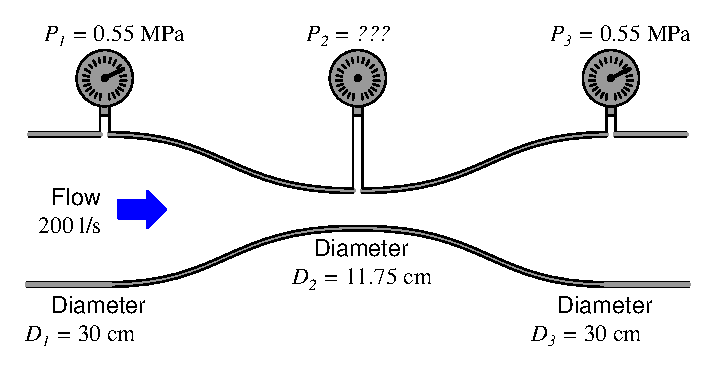
\includegraphics[width=15.5cm]{i00452x01.eps}$$

Bernoullis formel:

\vskip 10pt

$$z_1 \rho g + {v_1^2 \rho \over 2} + P_1 = z_2 \rho g + {v_2^2 \rho \over 2} + P_2$$


\noindent
Der,

$z$ = høyde av fluid, i meter (m)

$\rho$ = massetetthet av fluid, i kilogram per kubikkmeter (kg/m$^3$)

$g$ = tyngdeakselerasjon (9.81 m/s$^{2}$)

$v$ = hastighet til fluidet i meter per sekund (m/s)

$P$ = trykket i fluidet i pascal (Pa = N/m$^2$)

\vskip 10pt

Til slutt: Regn ut differansetrykket i dette venturi-måleelementet ($\Delta P$).

\vskip 10pt

\vskip 20pt \vbox{\hrule \hbox{\strut \vrule{} {\bf Forslag til sokratisk diskusjon} \vrule} \hrule}

\begin{itemize}
\item{} Læreboken skisserer en generell strategi for å lage en løsningsplan når man arbeider med komplekse matematiske formler. Strategien innebærer blant annet å skrive opp formlene og koble variabler mellom formler med piler. Forklar hvordan denne strategien fungerer, og vis hvordan den kan brukes på denne oppgaven.
\item{} En nyttig strategi i Bernoulli-oppgaver er å lage en tabell med hvert av «head»-leddene i ligningen. Forklar hvorfor dette er nyttig i denne typen oppgaver.
\item{} Når vi kjenner fluidhastigheten ($v$) i ett punkt i røret, finnes det en enkel måte å finne hastigheten i et annet punkt ved hjelp av forholdet mellom rørdiametrene? Her er for eksempel diameterforholdet mellom hals og innløp 5:12. Hvordan kan dette forholdet brukes for raskt å bestemme hastigheten i ett punkt når hastigheten i et annet punkt er kjent?
\end{itemize}

\underbar{file i00452}
%(END_QUESTION)





%(BEGIN_ANSWER)

$P_2$ = 0.42 MPa

\vskip 10pt

Oppfølgingsoppgave: Beregn {\it differanse}trykket mellom enten $P_1$ eller $P_3$ og $P_2$.

%(END_ANSWER)





%(BEGIN_NOTES)

% No blank lines allowed between lines of an \halign structure!
% I use comments (%) instead, so Tex doesn't choke.

$$V_1=\frac{Q}{A_1}=\frac{0.2m^3/s}{\pi \frac{(0.3m)^2}{4}}=2.83m/s$$
$$V_2=\frac{Q}{A_2}=\frac{0.2m^3/s}{\pi \frac{(0.1175m)^2}{4}}=18.44m/s$$




$$\cancel{z_1 \rho g} + {v_1^2 \rho \over 2} + P_1 = \cancel{z_2 \rho g} + {v_2^2 \rho \over 2} + P_2$$
$$P_2={v_1^2 \rho \over 2} + P_1 - {v_2^2 \rho \over 2}=\frac{2.83m/s\cdot 800kg/m^3}{2}$$

En interessant øvelse er å doble strømningsraten og beregne $\Delta P$ på nytt. Da ser du at sammenhengen er kvadratisk: Dobbel strømning gir firedoblet differansetrykk.

%INDEX% Physics, dynamic fluids: Bernoulli's equation

%(END_NOTES)
